\chapter{Wizja}

Przyjęta na początku wizja aplikacji zakładała:

\begin{itemize}
	\item Możliwość obsługiwania wielu klientów jednocześnie.
	\item Potencjalną możliwość uruchamiania zadań planowania na zdalnych węzłach obliczeniowych.
	\item Zwracanie wyników planowania bezpośrednio do zleceniodawcy przez węzeł obliczeniowy, który w tym celu informował by nas o adresie, na który odsyłać wyniki.
\end{itemize}

Rusynek \ref{fig:wizja} przedstawia schemat osadzenia tworzonego serwisu w jego potencjalnych środowisku uruchomieniowym.
W realnej sytuacji oczywiście potencjalnych klientów może być $m$ a węzłów obliczeniowych $n$.

\begin{figure}[!h]
	\centering
	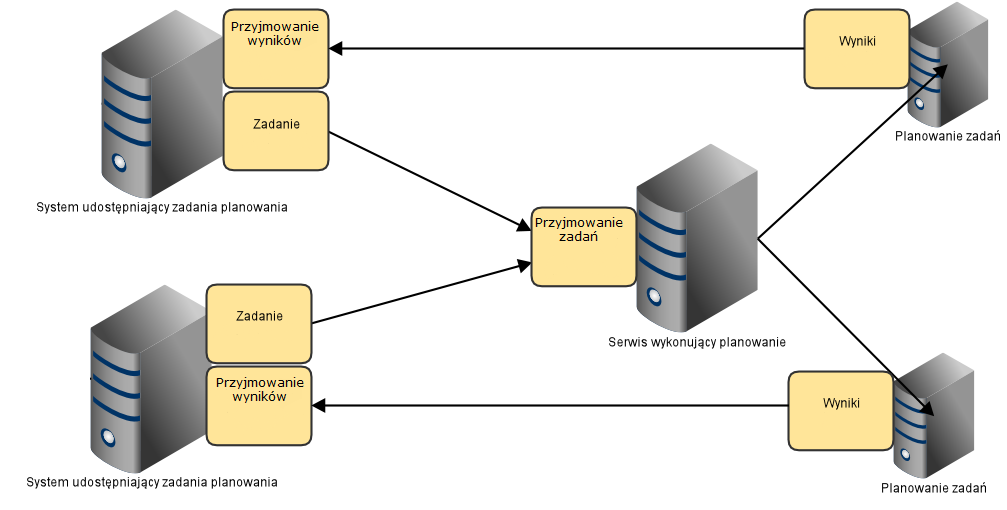
\includegraphics[width=\linewidth]{img/wizja}
	\caption{Wstępna wizja aplikacji i jej otoczenia.}
	\label{fig:wizja}
\end{figure}
